\begin{figure*}
    \newcommand*{\bheight}{8}
    \newcommand*{\loops}{6}
    \newcommand*{\bwidth}{0.2}
    \tikzset{
        aperture/.pic={
            \path [draw=black, rotate=#1, pattern=north east lines]
            (-3/4,-3/2) rectangle (3/4,3/2);
            \path [fill=white, draw=black, even odd rule]
            circle [radius=2/3] (-1,-1) rectangle (1,1);
        },
        barberpoll/.pic={
                \begin{axis}[
                    axis equal,  
                    % grid=both, 
                    view={270}{0}
                ]
                    \addplot3[
                        opacity = 0.7,
                        surf,
                        faceted color=gray,
                        lightgray,
                        samples = 25,
                        variable = \u,
                        variable y = \v,
                        domain = 0:360,
                        y domain = 0:\bheight] ({cos(u)}, {sin(u)}, {v});

                    \addplot3[
                        opacity = 1,
                        surf,
                        faceted color=none,
                        red,
                        samples = 25,
                        variable = \u,
                        variable y = \v,
                        domain = 160:270,
                        y domain = 0:\bheight
                    ] (
                    {cos(u)}, {sin(u)},
                    {
                            max(
                            ((\loops)*\bheight)/(\loops)-(\bwidth) + (\bheight)/(\loops)*0.5*cos(u/2),
                            min(
                            (\loops)*(\bheight)/(\loops)+(\bwidth)+(\bheight)/(\loops)*0.5*cos(u/2),
                            v
                            )
                            )
                        }
                    );

                    \foreach \loop in {2,...,\loops} {
                            \addplot3[
                                opacity =1,
                                surf,
                                faceted color=none,
                                red,
                                samples = 25,
                                variable = \u,
                                variable y = \v,
                                domain = 90:270,
                                y domain = 0:\bheight
                            ] (
                            {cos(u)}, {sin(u)},
                            {
                                    max(
                                    (((\loop)-1)*\bheight)/(\loops)-(\bwidth) +(\bheight)/(\loops)*0.5*cos(u/2),
                                    min(
                                    ((\loop)-1)*(\bheight)/(\loops)+(\bwidth) + (\bheight)/(\loops)*0.5*cos(u/2),
                                    v
                                    )
                                    )
                                }
                            );
                        }

                    \addplot3[
                        opacity = 1,
                        surf,
                        faceted color=none,
                        red,
                        samples = 25,
                        variable = \u,
                        variable y = \v,
                        domain = 90:200,
                        y domain = 0:\bheight
                    ] (
                    {cos(u)}, {sin(u)},
                    {
                            max(
                            ((0)*\bheight)/(\loops)-(\bwidth) +(\bheight)/(\loops)*0.5*cos(u/2),
                            min(
                            (0)*(\bheight)/(\loops)+(\bwidth)+(\bheight)/(\loops)*0.5*cos(u/2),
                            v
                            )
                            )
                        }
                    );
                \end{axis}
            }
    }
    \centering
    \begin{subfigure}[b]{0.3\textwidth}
        \centering
        \begin{adjustbox}{height=\textwidth}
            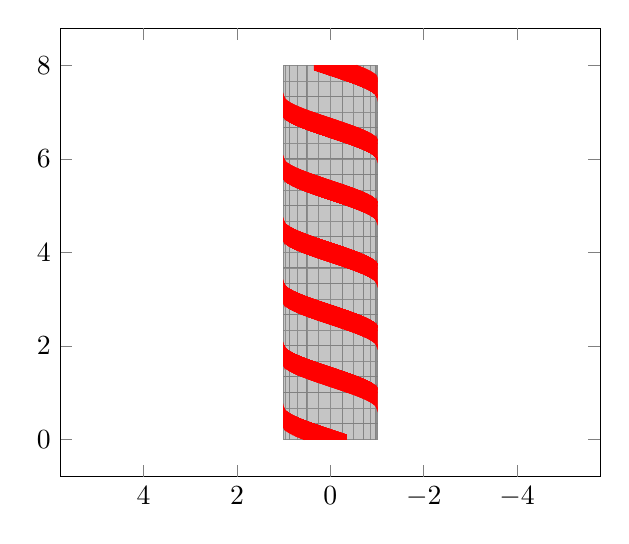
\begin{tikzpicture}
                \pic {barberpoll};
            \end{tikzpicture}
        \end{adjustbox}
        \caption{}
        \label{fig:y equals x}
    \end{subfigure}
    \hfill
    \begin{subfigure}[b]{0.3\textwidth}
        \centering
        \raisebox{22pt}{
            \begin{adjustbox}{height=\textwidth}
                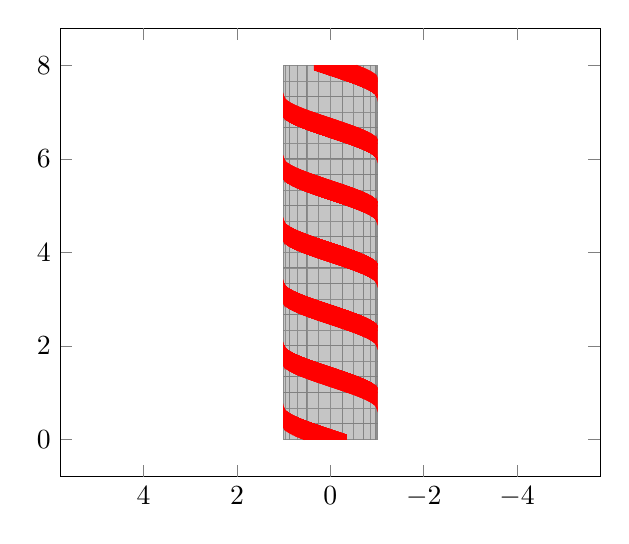
\begin{tikzpicture}
                    \pic {barberpoll};
                \end{tikzpicture}
            \end{adjustbox}
        }
        \caption{\(y=3sinx\)}
        \label{fig:three sin x}
    \end{subfigure}
    \hfill
    \begin{subfigure}[b]{0.3\textwidth}
        \centering
        \begin{adjustbox}{height=\textwidth}
            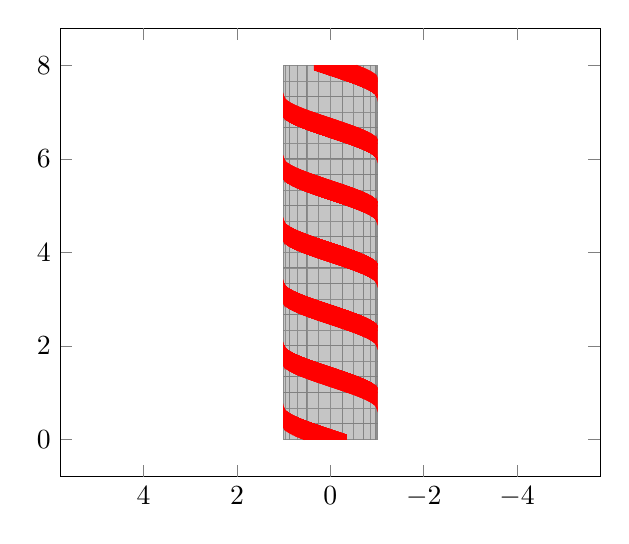
\begin{tikzpicture}
                \pic {barberpoll};
            \end{tikzpicture}
        \end{adjustbox}
        \caption{\(y=5/x\)}
        \label{fig:five over x}
    \end{subfigure}
    \caption{Three simple graphs.}
    \label{fig:three graphs}
\end{figure*}